% Compile with Tectonic or XeLaTeX.
\documentclass[final]{beamer}

% ====================
% Packages
% ====================
\usepackage[T1]{fontenc}
\usepackage[utf8]{inputenc}
\usepackage{lmodern}
\usepackage[size=custom,width=91.44,height=60.96,scale=0.78]{beamerposter}

\usetheme{gemini}
\usecolortheme{stanford}

\usepackage{graphicx}
\usepackage{booktabs}
\usepackage{array}
\usepackage{amsmath,amssymb}
\usepackage{ragged2e}
\usepackage{tikz}
\usepackage{xcolor}
\usetikzlibrary{arrows.meta,positioning,calc}

% ====================
% Layout
% ====================
\newlength{\sepwidth}
\newlength{\colwidth}
\setlength{\sepwidth}{0.025\paperwidth}
\setlength{\colwidth}{0.30\paperwidth}
\newcommand{\separatorcolumn}{\begin{column}{\sepwidth}\end{column}}

\renewcommand{\arraystretch}{1.12}
\newcommand{\metric}[1]{\textbf{#1}}
\newcommand{\sys}[1]{\texttt{#1}}
\newcommand{\figcap}[1]{%
  \vspace{-0.35em}%
  \begin{center}
  \begin{minipage}{0.96\linewidth}
  \centering{\small\color{coolgray}#1}
  \end{minipage}
  \end{center}
  \vspace{-0.45em}%
}

% ====================
% Title
% ====================
\title{From Text to Torque: Feasibility-Aware Tracking of Text-Generated Humanoid Motions}
\author{Kuzey Kantarcioglu \and Benji Warburton}
\institute[shortinst]{CS224R: Deep Reinforcement Learning \samelineand Stanford University}

\footercontent{
  \hfill
  Project repo: \sys{github.com/kuzeykantarcioglu/text-to-torque}
  \hfill
}

% ====================
% Document
% ====================
\begin{document}

\addtobeamertemplate{headline}{}%
{
    \begin{tikzpicture}[remember picture,overlay]
      \node[anchor=north east, inner sep=2.5cm]
      at ([xshift=0cm,yshift=1.8cm]current page.north east)
      {
\includegraphics[height=6.2cm]{stanford_logos/Block_S_2_color.png}};
    \end{tikzpicture}
}

\begin{frame}[t]

\begin{alertblock}{Main finding}
\large
Text-generated humanoid motion is stochastic enough that \textbf{reference choice becomes an RL intervention}. 
Before running expensive PPO, cheap motion diagnostics can select generated seeds that are easier to track physically.
\textbf{Diagnostic-best references beat diagnostic-worst references on jump, roll, and squat strict-PPO probes.}
\end{alertblock}

\vspace{-0.6em}
\begin{columns}[t]
\separatorcolumn

% =========================================
% Column 1
% =========================================
\begin{column}{\colwidth}

\begin{block}{Problem: plausible motion is not physical control}
\justifying
Text-to-motion models can generate convincing kinematic humanoid clips, but a torque-controlled Unitree G1 policy must satisfy contacts, gravity, balance, joint limits, and termination thresholds.

\vspace{0.35em}
\textbf{Research question:} which properties of a text-generated reference motion predict whether PPO can learn a stable tracking policy? We treat the generator as a stochastic proposal distribution over references, not as a guaranteed controller.
\end{block}

\begin{block}{Hypothesis: a reference feasibility boundary}
\justifying
PPO succeeds when the generated reference lies inside a reachable tracking basin. It fails when the kinematic target asks for states or contacts that the robot cannot realize under torque, balance, and termination constraints.

\vspace{0.2em}
\small
\begin{tabular}{>{\raggedright\arraybackslash}p{0.34\linewidth} >{\raggedright\arraybackslash}p{0.57\linewidth}}
\toprule
Reference signal & Expected PPO symptom \\
\midrule
root / joint acceleration spikes & high action-rate cost, falls, poor velocity tracking \\
bad contact or body pose & self-collisions, early terminations, low body-pose reward \\
large seed-to-seed variation & best-of-N selection should improve learnability \\
mostly speed-limited failure & temporal retiming should help \\
\bottomrule
\end{tabular}
\end{block}

\begin{block}{System pipeline}
\centering
\begin{tikzpicture}[
  node distance=0.55cm and 0.42cm,
  box/.style={draw=black, thick, rounded corners=3pt, fill=white, minimum height=1.05cm, align=center, inner sep=5pt},
  accent/.style={draw=cardinalred, thick, rounded corners=3pt, fill=cardinalred!7, minimum height=1.05cm, align=center, inner sep=5pt},
  arrow/.style={-{Latex[length=2.8mm]}, thick},
  every node/.style={font=\small}
]
\node[box, minimum width=3.0cm] (prompt) {Text prompt};
\node[accent, right=of prompt, minimum width=3.4cm] (kimodo) {Kimodo /\\KimoLab};
\node[box, right=of kimodo, minimum width=3.3cm] (refs) {$N$ reference\\seeds};

\node[accent, below=0.75cm of kimodo, minimum width=3.8cm] (diag) {Pre-RL\\diagnostics};
\node[box, left=of diag, minimum width=3.0cm] (select) {Best / worst\\seed selection};
\node[box, right=of diag, minimum width=3.5cm] (ppo) {MuJoCo Warp\\PPO tracking};

\draw[arrow] (prompt) -- (kimodo);
\draw[arrow] (kimodo) -- (refs);
\draw[arrow] (refs) -- (diag);
\draw[arrow] (diag) -- (select);
\draw[arrow] (select) -- (ppo);
\end{tikzpicture}

\vspace{0.7em}
\justifying
We run KimoLab on Modal GPUs, convert generated CSV motions to MuJoCo reference trajectories, and train PPO policies to track them in simulation.
\end{block}

\begin{block}{Reference motions before physics}
\centering
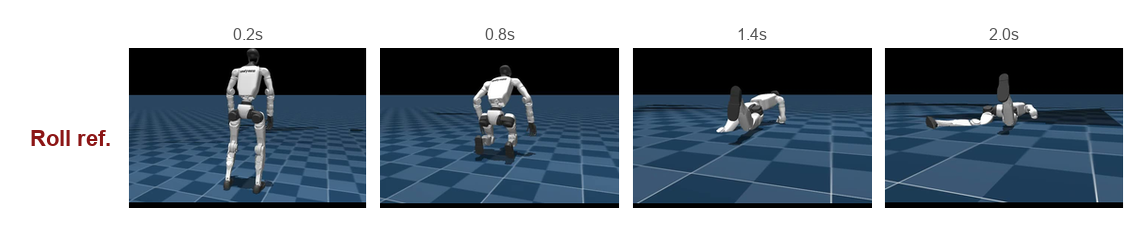
\includegraphics[width=\linewidth,height=4.2cm,keepaspectratio]{assets/poster_hard_reference_strip.png}
\figcap{Generated references can look plausible while already containing balance, contact, or body-pose artifacts that downstream PPO must absorb.}
\end{block}

\begin{block}{Diagnostics before PPO}
\justifying
For each generated motion, we compute cheap reference-only features:
\begin{itemize}
  \item root height range, root speed, root acceleration
  \item joint velocity and acceleration extrema
  \item body angular speed and initial-state feasibility checks
\end{itemize}

\vspace{-0.3em}
\centering
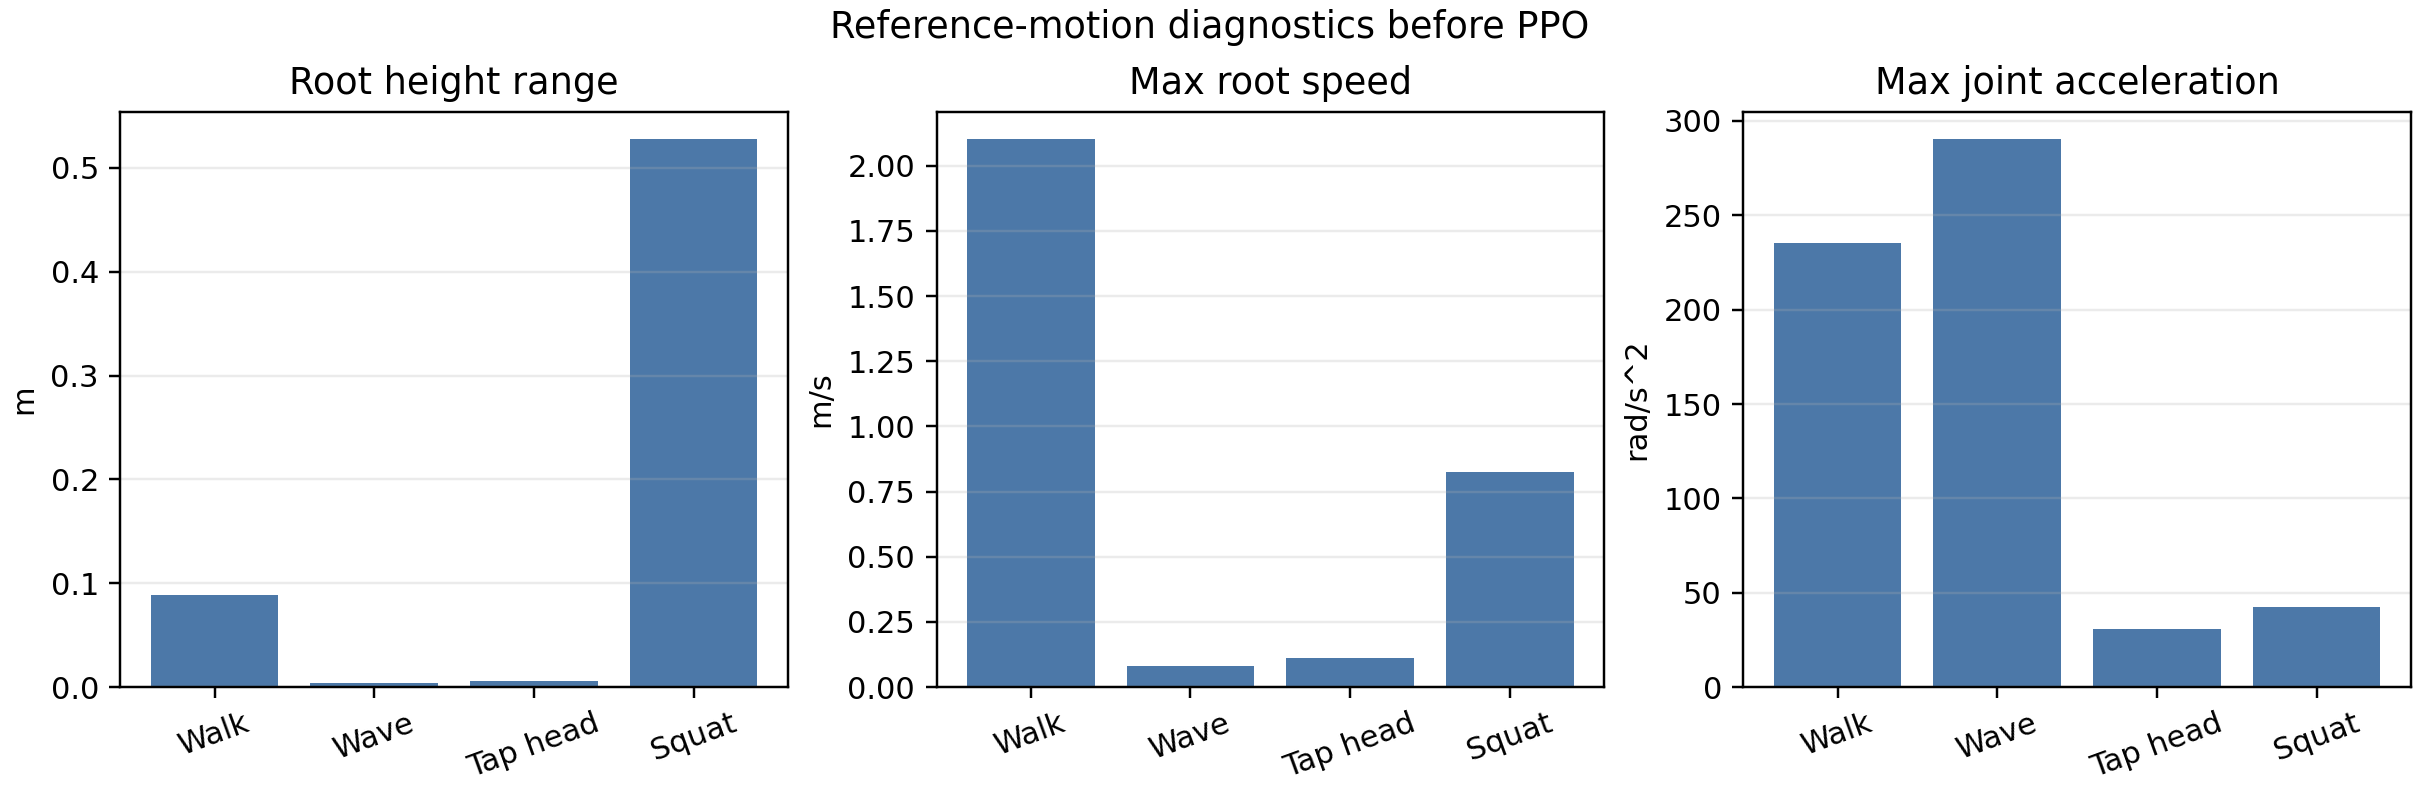
\includegraphics[width=\linewidth,height=4.2cm,keepaspectratio]{assets/final_reference_diagnostics.png}
\figcap{Diagnostics reveal that failure is not just "hard prompt" vs "easy prompt"; generated seeds vary materially within the same prompt.}
\end{block}

\end{column}

\separatorcolumn

% =========================================
% Column 2
% =========================================
\begin{column}{\colwidth}

\begin{block}{Best-of-N reference selection}
\justifying
For each prompt, generate 3--5 motion seeds, score every reference before PPO, then compare strict-PPO probes for the diagnostic-best and diagnostic-worst seeds. This tests whether the generator's randomness can be exploited as a search space over feasible references.

\vspace{0.35em}
\centering
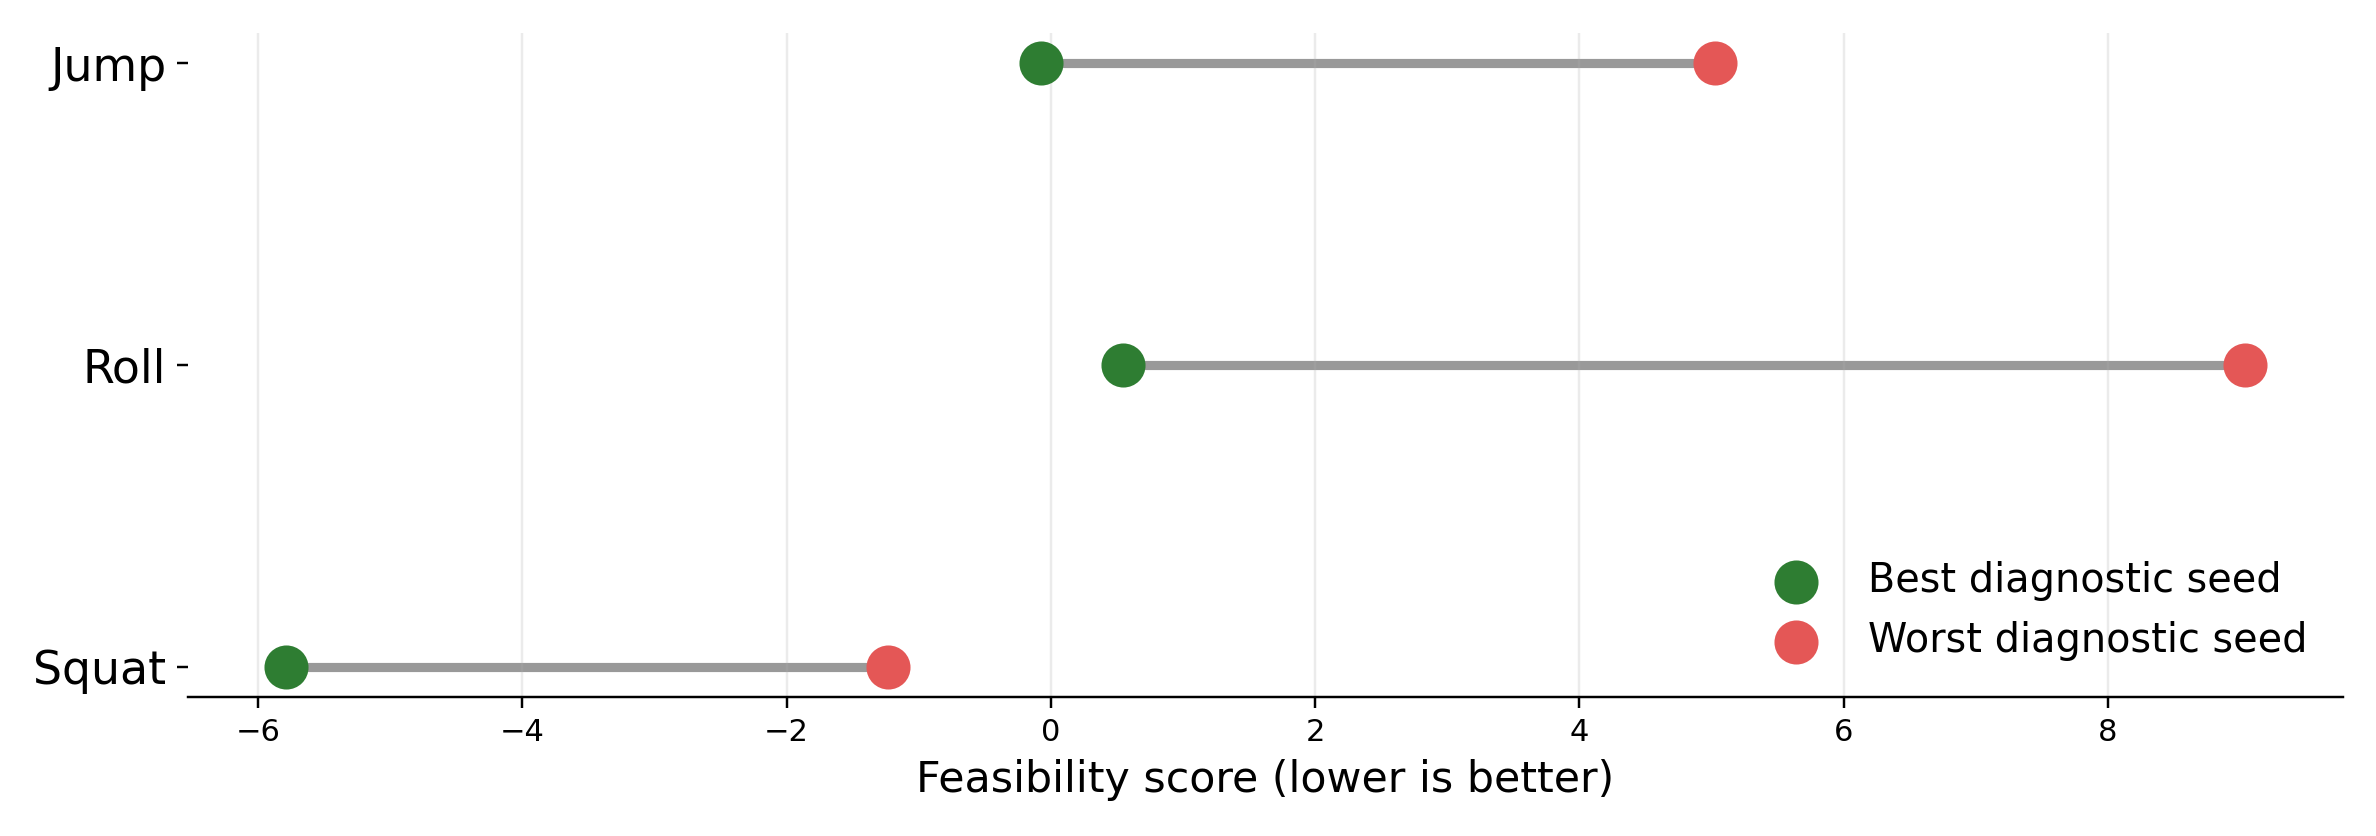
\includegraphics[width=\linewidth,height=5.8cm,keepaspectratio]{assets/poster_feasibility_spread.png}
\figcap{Lower feasibility score is better. Same prompt, different generated seed, very different reference feasibility.}

\justifying
The feasibility score is a clipped robust-z sum over reference-only diagnostics such as root acceleration and max joint acceleration. The point is not to learn a black-box predictor; it is to cheaply reject bad references before RL.
\end{block}

\begin{alertblock}{Result: diagnostics predict early learnability}
\centering
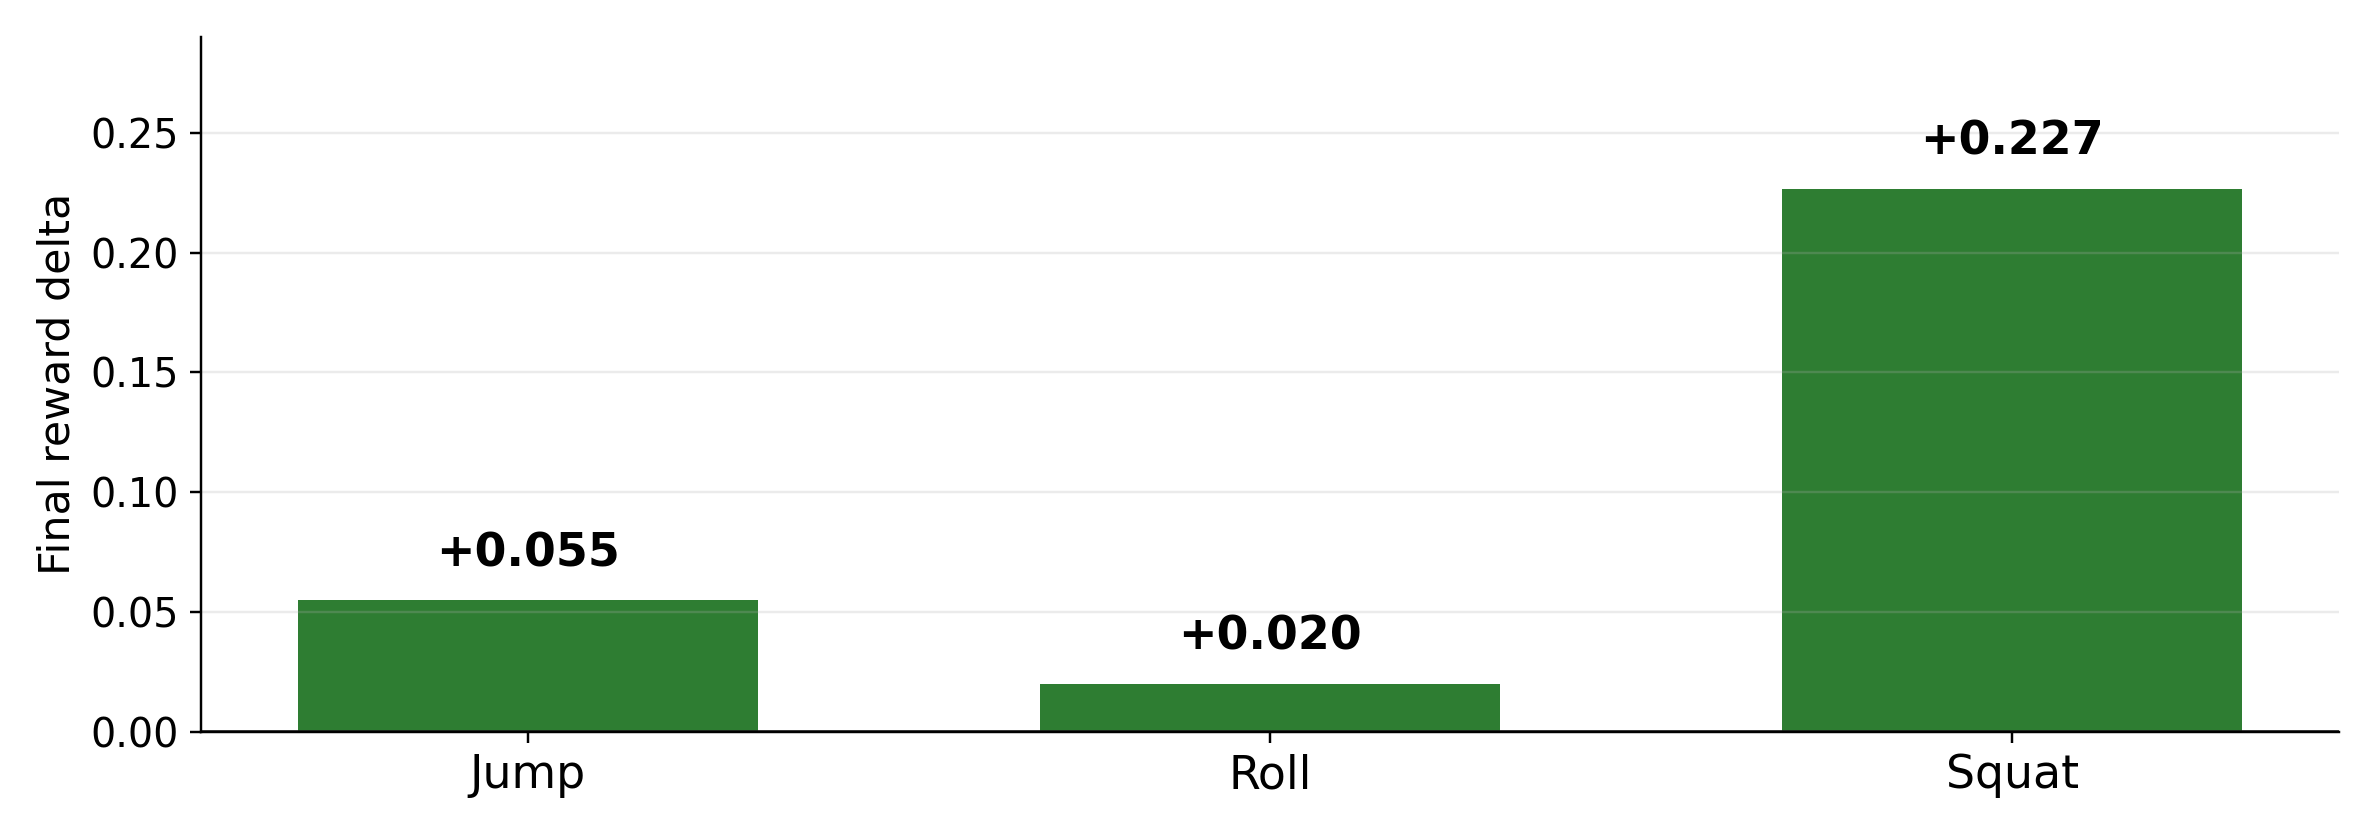
\includegraphics[width=\linewidth,height=6.7cm,keepaspectratio]{assets/poster_seed_delta.png}

\vspace{0.25em}
\small
\begin{tabular}{lccc}
\toprule
Motion & Best seed & Worst seed & Reward delta \\
\midrule
Jump  & 3 & 4 & $+0.055$ \\
Roll  & 3 & 1 & $+0.020$ \\
Squat & 3 & 1 & $\mathbf{+0.227}$ \\
\bottomrule
\end{tabular}

\vspace{0.2em}
\justifying
Diagnostic-best seeds improve strict-PPO reward on every tested motion. This supports the feasibility-boundary view: same prompt semantics, different generated dynamics, different PPO outcome. The practical recipe is simple: sample a few references, score them, and train the one most likely to be physically learnable.
\end{alertblock}

\begin{block}{Qualitative evidence}
\centering
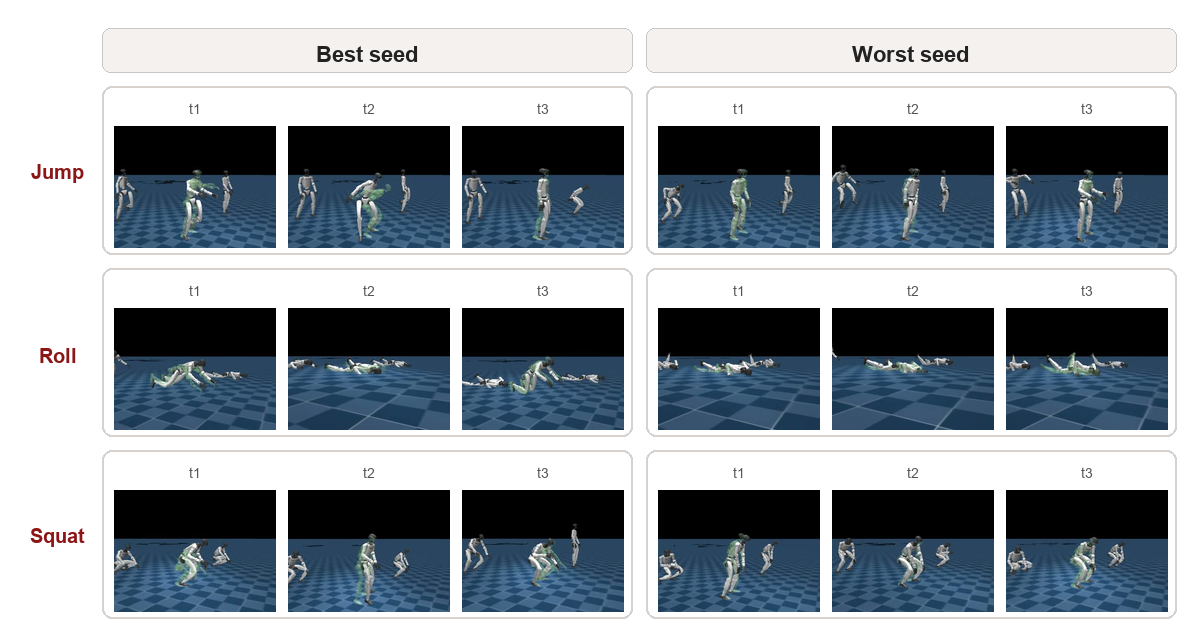
\includegraphics[width=\linewidth,height=10.0cm,keepaspectratio]{assets/poster_bestofn_rollouts.png}
\figcap{Three frames per rollout at the same probe horizon. Best and worst generated references produce visibly different early tracking behavior.}
\end{block}

\end{column}

\separatorcolumn

% =========================================
% Column 3
% =========================================
\begin{column}{\colwidth}

\begin{block}{Alternative repair: slow the reference}
\justifying
We also tested a temporal feasibility repair: take the diagnostic-worst seed and train strict PPO after slowing the reference to $2\times$ duration. This asks whether failures are mainly caused by excessive speed or torque demand.

\vspace{0.25em}
\centering
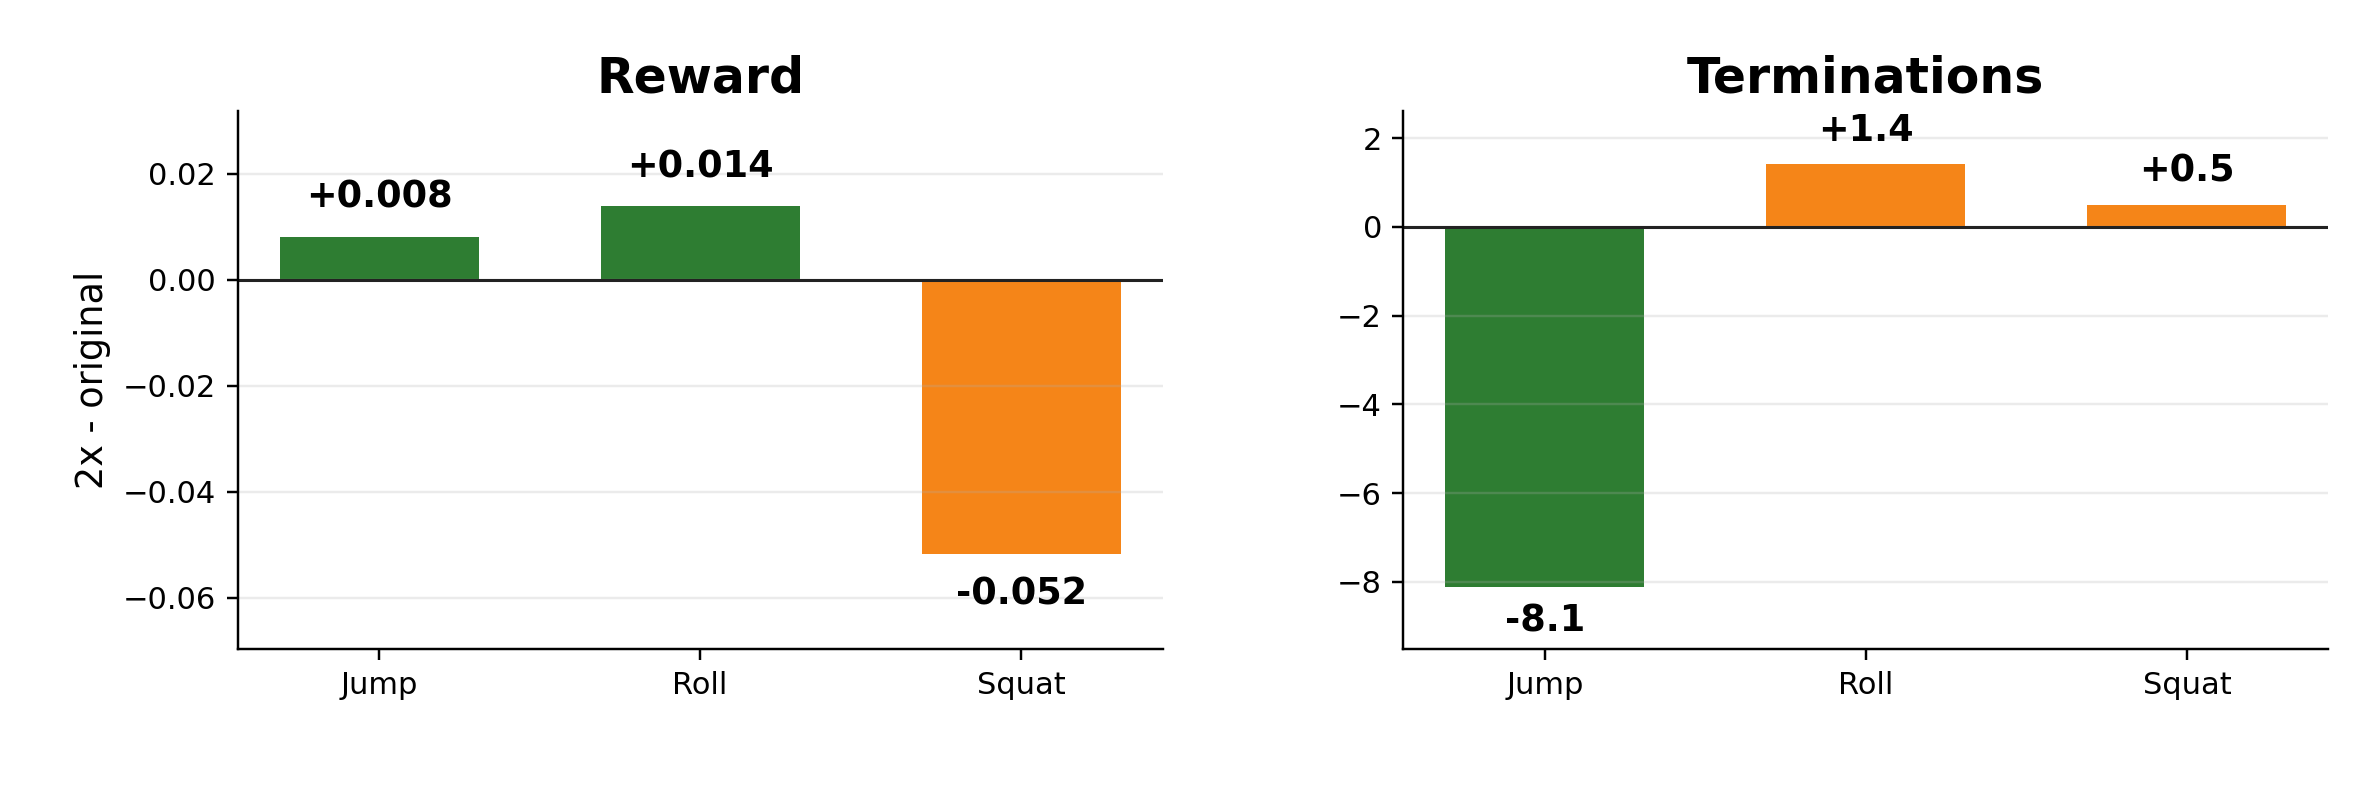
\includegraphics[width=\linewidth,height=4.8cm,keepaspectratio]{assets/poster_temporal_delta.png}

\vspace{-0.1em}
\small
\begin{tabular}{lccc}
\toprule
Motion & Reward delta & Termination delta & Verdict \\
\midrule
Jump  & $+0.008$ & $-8.125$ & slight help \\
Roll  & $+0.014$ & $+1.417$ & mixed \\
Squat & $-0.052$ & $+0.500$ & worse \\
\bottomrule
\end{tabular}

\vspace{0.25em}
\justifying
Naive retiming alone is not a reliable repair. It slightly helps jump and roll reward, but all slowed worst-seed runs still terminate early. This negative result matters: hard generated references are not only too fast; many also encode poor contacts or awkward body states.
\end{block}

\begin{block}{Rollouts: temporal repair is mixed}
\centering
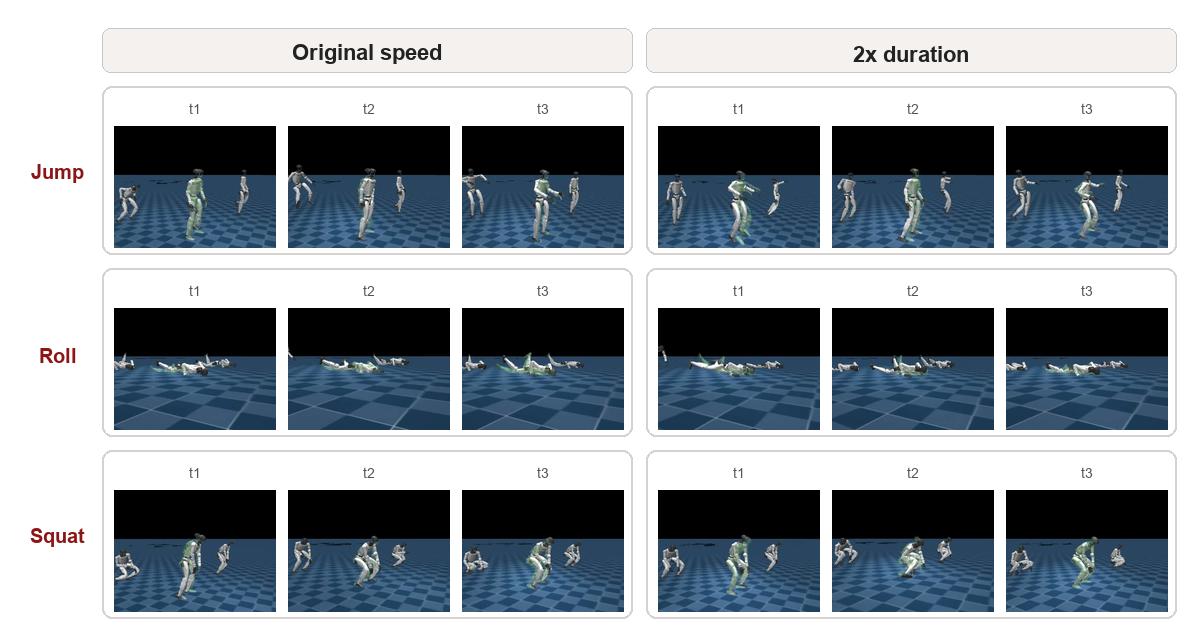
\includegraphics[width=\linewidth,height=8.2cm,keepaspectratio]{assets/poster_temporal_rollouts.png}
\figcap{Original-speed worst seeds vs $2\times$ slowed worst seeds. Retiming changes behavior, but does not solve the hard references.}
\end{block}

\begin{block}{Diagnostic-gated training recipe}
\scriptsize
\begin{tabular}{>{\raggedright\arraybackslash}p{0.32\linewidth} >{\raggedright\arraybackslash}p{0.60\linewidth}}
\toprule
Diagnosis & Action before expensive PPO \\
\midrule
Low feasibility score & run strict tracking baseline \\
Borderline score & compare strict vs loose/adaptive termination \\
High score or contact artifacts & regenerate seeds; avoid training on the worst sample \\
Large speed / acceleration spikes & test retiming as an ablation, not as the default fix \\
\bottomrule
\end{tabular}

\vspace{0.25em}
\justifying
The pipeline becomes a feasibility-aware loop: generate seeds, score them, choose the intervention, then spend GPU time.
\end{block}

\begin{block}{Experimental protocol}
\small
\begin{tabular}{>{\raggedright\arraybackslash}p{0.28\linewidth} >{\raggedright\arraybackslash}p{0.64\linewidth}}
\toprule
Suite & walk, wave, tap head, squat, jump, roll, acrobatic references \\
Probe & 150 strict-PPO iterations, 256 parallel environments \\
Metrics & reward, tracking errors, episode length, terminations, videos \\
\bottomrule
\end{tabular}
\end{block}

\begin{alertblock}{Takeaways}
\small
\justifying
\begin{itemize}
  \item Text-to-motion quality should be evaluated by \metric{downstream physical learnability}, not only visual plausibility.
  \item Best-of-N reference selection is cheap, simple, and improved all tested strict-PPO probes.
  \item Naive temporal repair is mixed; bad generated references often need regeneration or adaptive training, not just slower playback.
  \item Main demo message: reference generation is part of the RL algorithm, not a preprocessing detail.
\end{itemize}
\end{alertblock}

\end{column}

\separatorcolumn
\end{columns}
\end{frame}

\end{document}
